\chapter{System Design}

\section{Design Approach}
A design approach is a general philosophy that may or may not include a guide for specific methods. Some are to guide the overall goal of the design. Other approaches are to guide the tendencies of the designer. A combination of approaches may be used if they don't conflict.\\
\emph{Function Oriented Design Approach:}\\
Function Oriented Design Approach is partitioning of a design into subsystems and modules, with each one handling one or more functions. Contrast with object-oriented design, data-structure-oriented design. \\

This application project uses function oriented design approach. Every module and sub modules are made, based on their functionality.
These modules are designed and implemented separately and then they are integrated together to form the desired application.

\section{Detail Design}
The detailed design of this application is as follow:
\begin{enumerate}
\item \textbf{\emph{Registering a User:}}\\
The first step in this application is to get the users registered to both GCM Server and to Remote Web Server. For this, user will provide all the necessary details and press the register button. The request will first go to Google Cloud Messaging Server. GCM Server will provide
the registration id for that device. After that, all the information along with registration id is stored on Web Server and the user gets registered.

\item \textbf{\emph{User Login:}}\\
After registering, the user is allowed to log in. Username and password after validating at client side, is sent to server side to authentication. After authentication response is sent by the server to client, and then user gets logged in.

\item \textbf{\emph{Viewing the Notices:}}\\
At the first time, when you are using this application for the first time, it will fetch all the notices from server. In all the other case, all previous notices are fetched from application's own database stored inside client mobile. It then checks for new notices from the server. 
If there are new notices on the server, it will fetch all those notices.

\item \textbf{\emph{Searching a Notice:}}\\
The user is able to search the notice in listview depending on the title of the notice. It helps user to get the desired notice instantly.

\item \textbf{\emph{Deleting a Notice:}}\\
If the user does not want some notices, he/she can delete it from their phone. There will be no effect on server entry.

\item \textbf{\emph{Posting a Notice:}}\\
If a user is an admin, he is able to post the notice. In order to post the notices, he has three option. One option is that, he can post a simple text notice. Another option allows him to send some attachment image with the notice. In this, he has two options.
Either he can pick the image from the gallery or he can click a picture on the spot by using camera.
After that, press the post button to post the notice.

\item \textbf{\emph{Notification Buzz:}}\\
As soon as the admin post a notice, the script will run with which request is made by GCM Server to WebServer for all the registered IDs.
After getting all the registered IDs, notification is sent to all the users registered with this application.
Notification has a tune and vibration that runs whenever there is a notification received by the user from GCM Server.

\item \textbf{\emph{Reset Password:}}\\
This application also has the facility to reset the password. If one user has forgot his passwor, he/she can rest the password by giving
his username or email address. The user will be given a page in which he can set his new password. Forgotten password will be updated with the new one on the server.

\end{enumerate}

\begin{figure}[H]
\centering 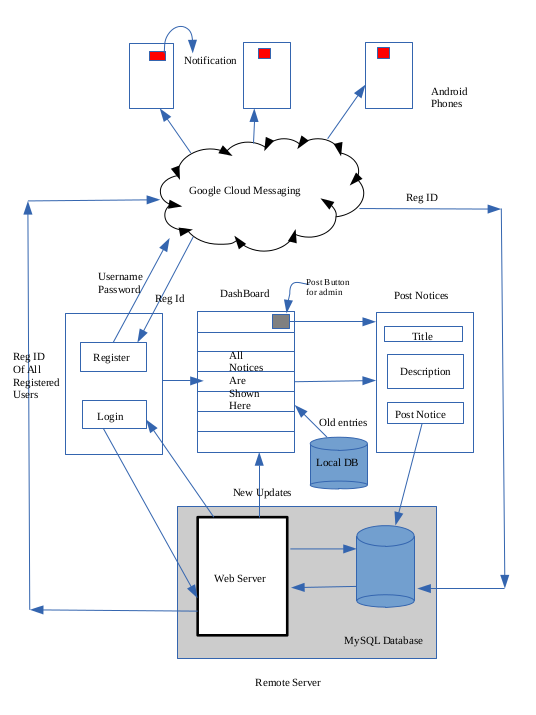
\includegraphics[scale=0.9]{image/detaildesign.png}
\caption{Detailed Design}
\end{figure}
\pagebreak

\section{System Design}
The system design can be clearly explained from the following diagrams:
\textbf{\emph{Use Case Diagram:}}\\

A Use Case diagram at its simplest is a representation of a user's interaction with the system and depicting the specifications of a use case. A use case diagram can portray the different types of users of a system and the various ways that they interact with the system. This type of diagram is typically used in conjunction with the textual use case and will often be accompanied by other types of diagrams as well.
\\
There are two types of user in this application, user and admin. Following depits their use case diagram:

\begin{figure}[H]
\centering 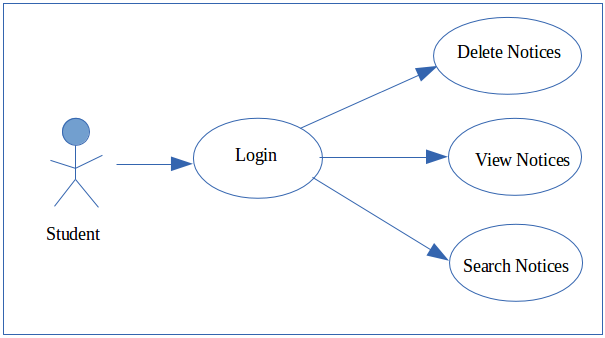
\includegraphics[scale=0.5]{image/usecase1.png}
\caption{Use Case Diagram For User}
\end{figure}

This diagram is showing what a normal user can do with this application. The user can login, after that he can view the notices, delete the notices and can search for particular notices.

\begin{figure}[H]
\centering 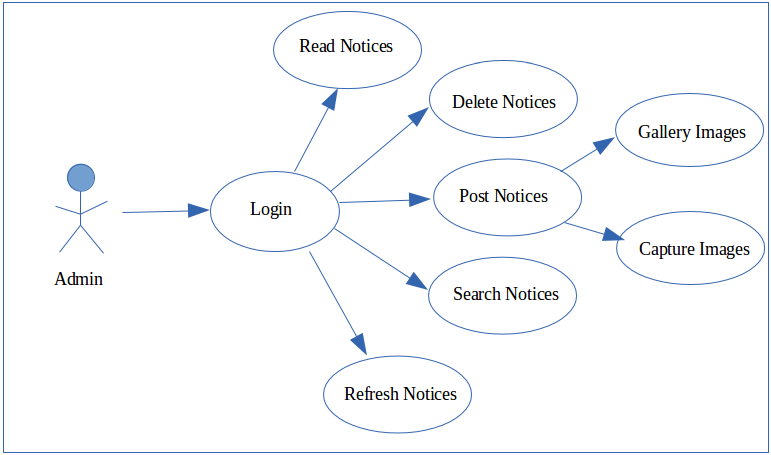
\includegraphics[scale=0.5]{image/usecase2.png}
\caption{Use Case Diagram For Admin}
\end{figure}

This diagram shows the priveleges of admin. An admin can post the notice in addition to viewing and deleting it. He can also post images as an attachment to the notices. Images can be choosen from the gallery or he can click the picture instantly usinng this application.






%%%%%%%%%%%%%%%%%%%%%%%%%%%%%%%%%%%%%%%%%%%%%%%%%%%%%%%%%%%%%%%%%%%%%%%%%%%%%%%%%%%%%%%%%%%%%%%%%%%%%%%%%%%%%%%%%%%%%%%%%%%%%%%%%
\pagebreak
\section{User Interface Design}
User Interface Design means the design of application with  which the user interacts. So it should be kept in mind that UI should be very simple and easy to use. It should be simple enough in look and feel also.
\begin{figure}[H]
\centering 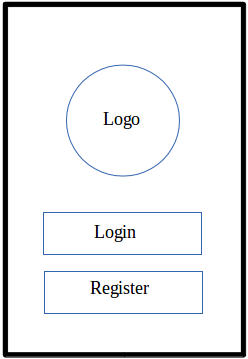
\includegraphics[scale=0.5]{image/ui1.png}
\caption{Landing Page}
\end{figure}

This page is the first page which is presented to the user. It has two buttons, to login or to register.

\begin{figure}[H]
\centering 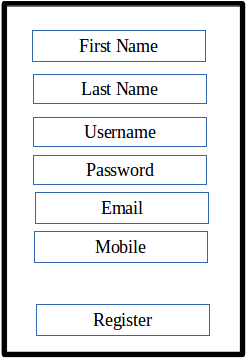
\includegraphics[scale=0.5]{image/ui2.png}
\caption{Registration Page}
\end{figure}

This is the registration page where the user get himself registered with the servers of this application.

\begin{figure}[H]
\centering 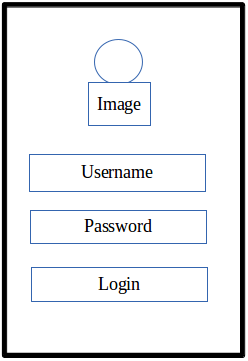
\includegraphics[scale=0.5]{image/ui3.png}
\caption{Login Page}
\end{figure}

This is the login page where user enters his username and password in order to access the notices.

\begin{figure}[H]
\centering 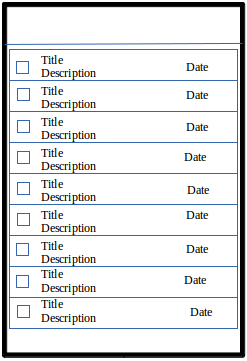
\includegraphics[scale=0.5]{image/ui4.png}
\caption{Dashboard Of Notices}
\end{figure}

This is the main dashboard, which receives all the notices from the user. The user can click on any notice, to see its details.
In addition to it, user can search and delete the notices.

\begin{figure}[H]
\centering 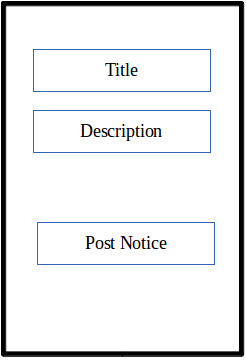
\includegraphics[scale=0.5]{image/ui5.png}
\caption{Post Notice Page}
\end{figure}

This page is only for the admin. Only admin can post the notices. He can choose images as attachment to notices.

\begin{figure}[H]
\centering 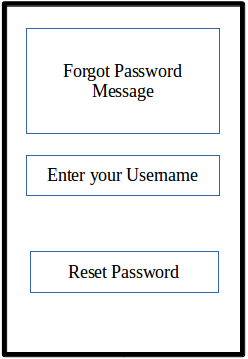
\includegraphics[scale=0.5]{image/ui6.png}
\caption{Reset Password Page}
\end{figure}

This is Reset Password page where the user can reset the password in order if he forgots his password.

%%%%%%%%%%%%%%%%%%%%%%%%%%%%%%%%%%%%%%%%%%%%%%%%%%%%%%%%%%%%%%%%%%%%%%%%%%%%%%%%%%%%%%%%%%%%%%%%%%%%%%%%%%%%%%%%%%%%%%%%%%%%%%
\pagebreak
\section{Database Design}
Database design is the process of producing a detailed data model of a database. This logical data model contains all the needed logical and physical design choices and physical storage parameters needed to generate a design in a data definition language, which can then be used to create a database. A fully attributed data model contains detailed attributes for each entity.\\

The term database design can be used to describe many different parts of the design of an overall database system. Principally, and most correctly, it can be thought of as the logical design of the base data structures used to store the data. In the relational model these are the tables and views. In an object database the entities and relationships map directly to object classes and named relationships. However, the term database design could also be used to apply to the overall process of designing, not just the base data structures, but also the forms and queries used as part of the overall database application within the database management system (DBMS).\\

The process of doing database design generally consists of a number of steps which will be carried out by the database designer. Usually, the designer must:
\begin{itemize}
\item Determine the relationships between the different data elements.
\item Superimpose a logical structure upon the data on the basis of these relationships.
\end{itemize}

\textbf{\emph{Design process}}
\begin{enumerate}

\item Determine the purpose of the database - This helps prepare for the remaining steps.
\item Find and organize the information required - Gather all of the types of information to record in the database, such as product name and order number.
\item Divide the information into tables - Divide information items into major entities or subjects, such as Products or Orders. Each subject then becomes a table.
\item Turn information items into columns - Decide what information needs to be stored in each table. Each item becomes a field, and is displayed as a column in the table. For example, an Employees table might include fields such as Last Name and Hire Date.
\item Specify primary keys - Choose each table’s primary key. The primary key is a column, or a set of columns, that is used to uniquely identify each row. An example might be Product ID or Order ID.
\item Set up the table relationships - Look at each table and decide how the data in one table is related to the data in other tables. Add fields to tables or create new tables to clarify the relationships, as necessary.
\item Refine the design - Analyze the design for errors. Create tables and add a few records of sample data. Check if results come from the tables as expected. Make adjustments to the design, as needed.
\item Apply the normalization rules - Apply the data normalization rules to see if tables are structured correctly. Make adjustments to the tables
\end{enumerate}

\subsection{ER Diagrams}
 An ER diagram is a diagram that helps to design databases in an efficient way.Attributes in ER diagrams are usually modeled as an oval with the name of the attribute, linked to the entity or relationship that contains the attribute.\\

Within the relational model the final step can generally be broken down into two further steps, that of determining the grouping of information within the system, generally determining what are the basic objects about which information is being stored, and then determining the relationships between these groups of information, or objects. \\

An Entity Relationship Diagram (ERD) is a visual representation of different data using conventions that describe how these data are related to each other. ER diagrams are most often associated with complex databases that are used in software engineering and IT networks. In particular, ER diagrams are frequently used during the design stage of a development process in order to identify different system elements and their relationships with each other. For example, an inventory software used in a retail shop will have a database that monitors elements such as purchases, item, item type, item source and item price.\\
The ER diagram of database used in the project is as follow:
\begin{figure}[H]
\centering 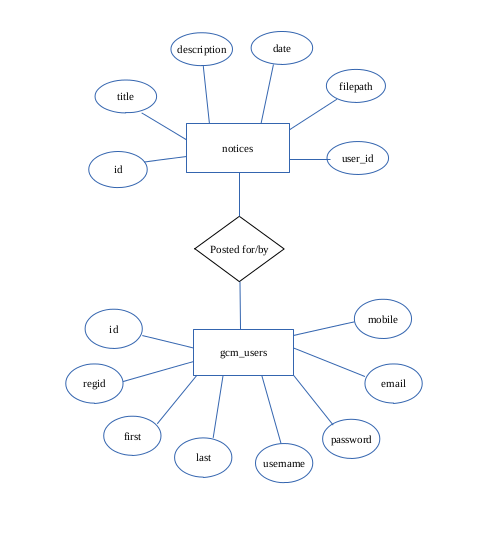
\includegraphics[scale=0.9]{image/erdiagram.png}
\caption{ER Diagram}
\end{figure}

\subsection{Normalization}
Normalization is a systematic way of ensuring that a database structure is suitable for general-purpose querying and free of certain undesirable characteristics—insertion, update, and deletion anomalies—that could lead to a loss of data integrity.
\\
A standard piece of database design guidance is that the designer should create a fully normalized design; selective denormalization can subsequently be performed, but only for performance reasons. However, some modeling disciplines, such as the dimensional modeling approach to data warehouse design, explicitly recommend non-normalized designs, i.e. designs that in large part do not adhere to 3NF. Normalization consists of normal forms that are 1NF, 2NF, 3NF, BOYCE-CODD NF (3.5NF), 4NF and 5NF.

\subsection{Database Manipulation}
Data Manipulation is retrieval of information from the database, insertion of new information into the database, deletion of information in the database modification of information in the database. A DML is a language which enables users to access and manipulate data.
The goal is to provide efficient human interaction with the system.\\

There are two types of DML:
\begin{enumerate}
\item \emph{Procedural:} In it, the user specifies what data is needed and how to get it.
\item \emph{Non Procedural:} In it, the user only specifies what data is needed. It is easier for user and may not generate code as efficient as that produced by procedural languages.
\end{enumerate}
 A query language is a portion of a DML involving information retrieval only. The terms DML and query language are often used synonymously. 
\subsection{Database Connection Control and Strings}
\begin{enumerate}
\item \textbf{\emph{Database connection control:}} It is a feature which prevents users from connecting to a database. This feature is also called passive shutdown because when connection control is invoked, users who are currently connected to the database remain unaffected until they disconnect. This capability is useful if you need to acquire exclusive access to a database to perform maintenance operations, such as compacting the database, or make updates to the database's design.\\

When connection control is invoked, users who are currently connected to a database remain unaffected until they disconnect from the database. At that point they will be unable to reconnect to the database until the user who invoked connection control revokes it or closes his or her connection to the database.\\

The following scenarios provide examples of how the connection control feature works. Assume there are five users in the database and that user five has invoked connection control on the database:\\

\textbf{Scenario 1} \\
User six tries to connect to the database, but is denied access, and an error message is returned stating that user five is preventing the database from being opened.

\textbf{Scenario 2} \\
User one closes the database and tries to reconnect to the database, but is denied access, and an error message is returned stating that user five is preventing the database from being opened.

\textbf{Scenario 3}\\
User five closes the database. User six tries to open the database and is successful. This is because connection control only persists while the user who invoked it remains connected to the database.

\textbf{Scenario 4}\\
Users one through four exit the database. User five uses the ADO OpenSchema method to retrieve a list of users in the database and determines that no other users are in the database. User five compacts the database, closes the database, and connection control is automatically revoked.

\item \textbf{\emph{Connection String:}} A connection string is a string that specifies information about a data source and the means of connecting to it. It is passed in code to an underlying driver or provider in order to initiate the connection. Whilst commonly used for a database connection, the data source could also be a spreadsheet or text file.

The connection string may include attributes such as the name of the driver, server and database, as well as security information such as user name and password.\\

\emph{Example of MySQL Connection String}\\
Server=myServerAddress;Port=1234;Database=myDataBase;Uid=myUsername;\\
Pwd=myPassword;\\

The port 3306 is the default MySql port. The value is ignored if Unix socket is used.
\end{enumerate}


%%%%%%%%%%%%%%%%%%%%%%%%%%%%%%%%%%%%%%%%%%%%%%%%%%%%%%%%%%%%%%%%%%%%%%%%%%%%%%%%%%%%%%%%%%%%%%%%%%%%%%%%%%%%%%%%%%%%%%%%%%%%%
\pagebreak
\section{Methodology}
The methodology used in project is Agile Software Development. Agile Software Development methodology is used especially for software development, that is characterized by the division of tasks into short phases of work and frequent reassessment and adaptation of plans.\\

It is for a project that needs extreme agility in requirements. The key features of agile are its short-termed delivery cycles (sprints), agile requirements, dynamic team culture, less restrictive project control and emphasis on real-time communication.\\

Agile software development is a group of software development methods based on iterative and incremental development, in which requirements and solutions evolve through collaboration between self-organizing, cross-functional teams. It promotes adaptive planning, evolutionary development and delivery, a time-boxed iterative approach, and encourages rapid and flexible response to change. It is a conceptual framework that promotes foreseen tight iterations throughout the development cycle.\\
\begin{figure}[H]
\centering 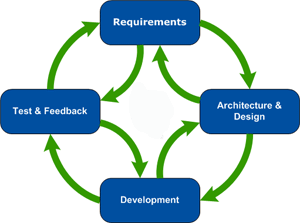
\includegraphics[scale=0.9]{image/agile.png}
\caption{Agile Software Development Methodology}
\end{figure}


The Manifesto of Agile Software Development context are:
\begin{itemize}
\item \emph{Individuals and interactions –} In agile development, self-organization and motivation are important, as are interactions like co-location and pair programming.
\item \emph{Working software –} Working software will be more useful and welcome than just presenting documents to clients in meetings.
\item \emph{Customer collaboration –} Requirements cannot be fully collected at the beginning of the software development cycle, therefore continuous customer or stakeholder involvement is very important.
\item \emph{Responding to change –} Agile development is focused on quick responses to change and continuous development.
\end{itemize}
